\begin{figure}[t]
\centering
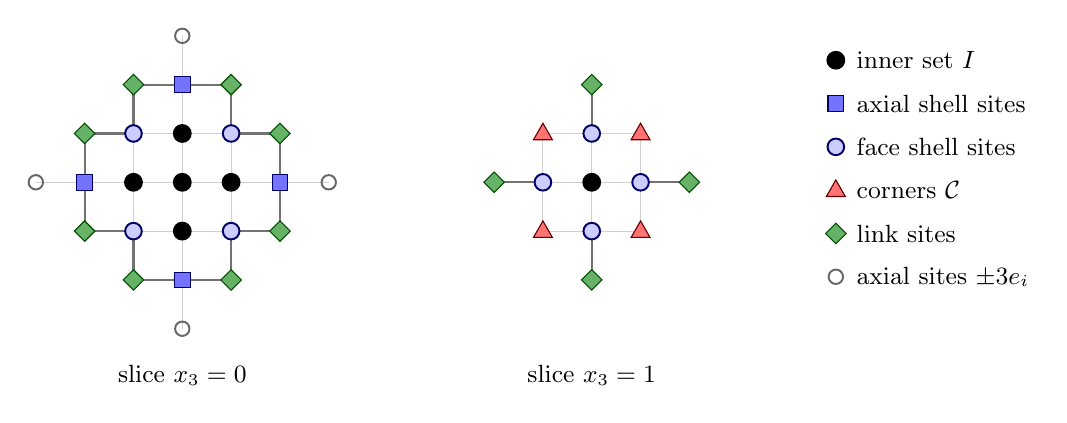
\begin{tikzpicture}[line cap=round]
\draw[black!18] (-1.860,0.000) -- (-1.240,0.000);
\draw[black!55,line width=0.8pt] (-1.240,-0.620) -- (-1.240,0.000);
\draw[black!55,line width=0.8pt] (-1.240,-0.620) -- (-0.620,-0.620);
\draw[black!55,line width=0.8pt] (-1.240,0.000) -- (-1.240,0.620);
\draw[black!18] (-1.240,0.000) -- (-0.620,0.000);
\draw[black!55,line width=0.8pt] (-1.240,0.620) -- (-0.620,0.620);
\draw[black!55,line width=0.8pt] (-0.620,-1.240) -- (-0.620,-0.620);
\draw[black!55,line width=0.8pt] (-0.620,-1.240) -- (0.000,-1.240);
\draw[black!18] (-0.620,-0.620) -- (-0.620,0.000);
\draw[black!18] (-0.620,-0.620) -- (0.000,-0.620);
\draw[black!18] (-0.620,0.000) -- (-0.620,0.620);
\draw[black!18] (-0.620,0.000) -- (0.000,0.000);
\draw[black!55,line width=0.8pt] (-0.620,0.620) -- (-0.620,1.240);
\draw[black!18] (-0.620,0.620) -- (0.000,0.620);
\draw[black!55,line width=0.8pt] (-0.620,1.240) -- (0.000,1.240);
\draw[black!18] (0.000,-1.860) -- (0.000,-1.240);
\draw[black!18] (0.000,-1.240) -- (0.000,-0.620);
\draw[black!55,line width=0.8pt] (0.000,-1.240) -- (0.620,-1.240);
\draw[black!18] (0.000,-0.620) -- (0.000,0.000);
\draw[black!18] (0.000,-0.620) -- (0.620,-0.620);
\draw[black!18] (0.000,0.000) -- (0.000,0.620);
\draw[black!18] (0.000,0.000) -- (0.620,0.000);
\draw[black!18] (0.000,0.620) -- (0.000,1.240);
\draw[black!18] (0.000,0.620) -- (0.620,0.620);
\draw[black!18] (0.000,1.240) -- (0.000,1.860);
\draw[black!55,line width=0.8pt] (0.000,1.240) -- (0.620,1.240);
\draw[black!55,line width=0.8pt] (0.620,-1.240) -- (0.620,-0.620);
\draw[black!18] (0.620,-0.620) -- (0.620,0.000);
\draw[black!55,line width=0.8pt] (0.620,-0.620) -- (1.240,-0.620);
\draw[black!18] (0.620,0.000) -- (0.620,0.620);
\draw[black!18] (0.620,0.000) -- (1.240,0.000);
\draw[black!55,line width=0.8pt] (0.620,0.620) -- (0.620,1.240);
\draw[black!55,line width=0.8pt] (0.620,0.620) -- (1.240,0.620);
\draw[black!55,line width=0.8pt] (1.240,-0.620) -- (1.240,0.000);
\draw[black!55,line width=0.8pt] (1.240,0.000) -- (1.240,0.620);
\draw[black!18] (1.240,0.000) -- (1.860,0.000);
\draw[black!60,line width=0.7pt] (-1.860,0.000) circle (2.6pt);
\filldraw[fill=green!50!black!60,draw=green!30!black] (-1.240,-0.620+0.13) -- (-1.240+0.13,-0.620) -- (-1.240,-0.620-0.13) -- (-1.240-0.13,-0.620) -- cycle;
\filldraw[fill=blue!55,draw=blue!40!black] (-1.240-0.10,0.000-0.10) rectangle (-1.240+0.10,0.000+0.10);
\filldraw[fill=green!50!black!60,draw=green!30!black] (-1.240,0.620+0.13) -- (-1.240+0.13,0.620) -- (-1.240,0.620-0.13) -- (-1.240-0.13,0.620) -- cycle;
\filldraw[fill=green!50!black!60,draw=green!30!black] (-0.620,-1.240+0.13) -- (-0.620+0.13,-1.240) -- (-0.620,-1.240-0.13) -- (-0.620-0.13,-1.240) -- cycle;
\filldraw[fill=blue!20,draw=blue!40!black,line width=0.7pt] (-0.620,-0.620) circle (3.0pt);
\fill[black] (-0.620,0.000) circle (3.4pt);
\filldraw[fill=blue!20,draw=blue!40!black,line width=0.7pt] (-0.620,0.620) circle (3.0pt);
\filldraw[fill=green!50!black!60,draw=green!30!black] (-0.620,1.240+0.13) -- (-0.620+0.13,1.240) -- (-0.620,1.240-0.13) -- (-0.620-0.13,1.240) -- cycle;
\draw[black!60,line width=0.7pt] (0.000,-1.860) circle (2.6pt);
\filldraw[fill=blue!55,draw=blue!40!black] (0.000-0.10,-1.240-0.10) rectangle (0.000+0.10,-1.240+0.10);
\fill[black] (0.000,-0.620) circle (3.4pt);
\fill[black] (0.000,0.000) circle (3.4pt);
\fill[black] (0.000,0.620) circle (3.4pt);
\filldraw[fill=blue!55,draw=blue!40!black] (0.000-0.10,1.240-0.10) rectangle (0.000+0.10,1.240+0.10);
\draw[black!60,line width=0.7pt] (0.000,1.860) circle (2.6pt);
\filldraw[fill=green!50!black!60,draw=green!30!black] (0.620,-1.240+0.13) -- (0.620+0.13,-1.240) -- (0.620,-1.240-0.13) -- (0.620-0.13,-1.240) -- cycle;
\filldraw[fill=blue!20,draw=blue!40!black,line width=0.7pt] (0.620,-0.620) circle (3.0pt);
\fill[black] (0.620,0.000) circle (3.4pt);
\filldraw[fill=blue!20,draw=blue!40!black,line width=0.7pt] (0.620,0.620) circle (3.0pt);
\filldraw[fill=green!50!black!60,draw=green!30!black] (0.620,1.240+0.13) -- (0.620+0.13,1.240) -- (0.620,1.240-0.13) -- (0.620-0.13,1.240) -- cycle;
\filldraw[fill=green!50!black!60,draw=green!30!black] (1.240,-0.620+0.13) -- (1.240+0.13,-0.620) -- (1.240,-0.620-0.13) -- (1.240-0.13,-0.620) -- cycle;
\filldraw[fill=blue!55,draw=blue!40!black] (1.240-0.10,0.000-0.10) rectangle (1.240+0.10,0.000+0.10);
\filldraw[fill=green!50!black!60,draw=green!30!black] (1.240,0.620+0.13) -- (1.240+0.13,0.620) -- (1.240,0.620-0.13) -- (1.240-0.13,0.620) -- cycle;
\draw[black!60,line width=0.7pt] (1.860,0.000) circle (2.6pt);
\node[font=\small] at (0.00,-2.45) {slice $x_3=0$};
\draw[black!55,line width=0.8pt] (3.960,0.000) -- (4.580,0.000);
\draw[black!18] (4.580,-0.620) -- (4.580,0.000);
\draw[black!18] (4.580,-0.620) -- (5.200,-0.620);
\draw[black!18] (4.580,0.000) -- (4.580,0.620);
\draw[black!18] (4.580,0.000) -- (5.200,0.000);
\draw[black!18] (4.580,0.620) -- (5.200,0.620);
\draw[black!55,line width=0.8pt] (5.200,-1.240) -- (5.200,-0.620);
\draw[black!18] (5.200,-0.620) -- (5.200,0.000);
\draw[black!18] (5.200,-0.620) -- (5.820,-0.620);
\draw[black!18] (5.200,0.000) -- (5.200,0.620);
\draw[black!18] (5.200,0.000) -- (5.820,0.000);
\draw[black!55,line width=0.8pt] (5.200,0.620) -- (5.200,1.240);
\draw[black!18] (5.200,0.620) -- (5.820,0.620);
\draw[black!18] (5.820,-0.620) -- (5.820,0.000);
\draw[black!18] (5.820,0.000) -- (5.820,0.620);
\draw[black!55,line width=0.8pt] (5.820,0.000) -- (6.440,0.000);
\filldraw[fill=green!50!black!60,draw=green!30!black] (3.960,0.000+0.13) -- (3.960+0.13,0.000) -- (3.960,0.000-0.13) -- (3.960-0.13,0.000) -- cycle;
\filldraw[fill=red!55,draw=red!40!black] (4.580,-0.620+0.13) -- (4.580-0.12,-0.620-0.08) -- (4.580+0.12,-0.620-0.08) -- cycle;
\filldraw[fill=blue!20,draw=blue!40!black,line width=0.7pt] (4.580,0.000) circle (3.0pt);
\filldraw[fill=red!55,draw=red!40!black] (4.580,0.620+0.13) -- (4.580-0.12,0.620-0.08) -- (4.580+0.12,0.620-0.08) -- cycle;
\filldraw[fill=green!50!black!60,draw=green!30!black] (5.200,-1.240+0.13) -- (5.200+0.13,-1.240) -- (5.200,-1.240-0.13) -- (5.200-0.13,-1.240) -- cycle;
\filldraw[fill=blue!20,draw=blue!40!black,line width=0.7pt] (5.200,-0.620) circle (3.0pt);
\fill[black] (5.200,0.000) circle (3.4pt);
\filldraw[fill=blue!20,draw=blue!40!black,line width=0.7pt] (5.200,0.620) circle (3.0pt);
\filldraw[fill=green!50!black!60,draw=green!30!black] (5.200,1.240+0.13) -- (5.200+0.13,1.240) -- (5.200,1.240-0.13) -- (5.200-0.13,1.240) -- cycle;
\filldraw[fill=red!55,draw=red!40!black] (5.820,-0.620+0.13) -- (5.820-0.12,-0.620-0.08) -- (5.820+0.12,-0.620-0.08) -- cycle;
\filldraw[fill=blue!20,draw=blue!40!black,line width=0.7pt] (5.820,0.000) circle (3.0pt);
\filldraw[fill=red!55,draw=red!40!black] (5.820,0.620+0.13) -- (5.820-0.12,0.620-0.08) -- (5.820+0.12,0.620-0.08) -- cycle;
\filldraw[fill=green!50!black!60,draw=green!30!black] (6.440,0.000+0.13) -- (6.440+0.13,0.000) -- (6.440,0.000-0.13) -- (6.440-0.13,0.000) -- cycle;
\node[font=\small] at (5.20,-2.45) {slice $x_3=1$};
\fill[black] (8.300,1.550) circle (3.4pt);
\node[right=4pt,font=\small] at (8.30,1.55) {inner set $I$};
\filldraw[fill=blue!55,draw=blue!40!black] (8.300-0.10,1.000-0.10) rectangle (8.300+0.10,1.000+0.10);
\node[right=4pt,font=\small] at (8.30,1.00) {axial shell sites};
\filldraw[fill=blue!20,draw=blue!40!black,line width=0.7pt] (8.300,0.450) circle (3.0pt);
\node[right=4pt,font=\small] at (8.30,0.45) {face shell sites};
\filldraw[fill=red!55,draw=red!40!black] (8.300,-0.100+0.13) -- (8.300-0.12,-0.100-0.08) -- (8.300+0.12,-0.100-0.08) -- cycle;
\node[right=4pt,font=\small] at (8.30,-0.10) {corners $\mathcal C$};
\filldraw[fill=green!50!black!60,draw=green!30!black] (8.300,-0.650+0.13) -- (8.300+0.13,-0.650) -- (8.300,-0.650-0.13) -- (8.300-0.13,-0.650) -- cycle;
\node[right=4pt,font=\small] at (8.30,-0.65) {link sites};
\draw[black!60,line width=0.7pt] (8.300,-1.200) circle (2.6pt);
\node[right=4pt,font=\small] at (8.30,-1.20) {axial sites $\pm3e_i$};
\end{tikzpicture}
\caption{Two horizontal slices of the neighbourhood of the origin used in \cref{sec:ordered}. The shell $\partial I=\{\|x\|_1=2\}$ separates the inner set $I$ from the exterior. Each link site of type $(2,1,0)$ joins one axial and one face shell site (dark bonds); summing over its spin couples the two shell spins and produces the factor $\xi^{d(b)}$ in~\eqref{eq:Psi}. The corners appear in the slices $x_3=\pm1$.}
\label{fig:shells}
\end{figure}
